\chapter{Sensitivity Analysis of the Radial Diffusion System}\label{app:psdSensitivity}

\section*{Model Sensitivity}

Sensitivity analysis originated from the need to quantify the effect that small errors in 
parameters of a partial differential equation (PDE) have on its solution. \citet{KODA1979259} 
described three approaches to sensitivity analysis of partial differential equations:
\begin{enumerate}
    \item the direct method,
    \item the variational method, and 
    \item the Fourier amplitude sensitivity test (FAST).
\end{enumerate}
They compared these techniques by applying them on the problem of atmospheric diffusion. 

Sensitivity of partial differential equations to their parameters has important implications for 
PDE constrained inverse problems. As a general rule, parameter identifiability increases with 
increasing sensitivity. For the Bayesian PDE inverse problem, this implies that posterior 
uncertainties of a parameter decrease if the forward model is sensitive to that parameter. 

In this appendix, we apply the direct method of sensitivity analysis on the radial diffusion 
system from \cref{sec:radDiffusionIntroduction} and visualise the sensitivity of the phase 
space density to the parameters of the diffusion field, the loss rate, and the source term.


\subsection*{Sensitivity: The Direct Method}

Consider the PDE system introduced in \cref{eq:forwardModel} 
\begin{equation}\label{eq:forwardModelPDE}
    \mathcal{L}_{\theta} f(x)  = q_{\theta}(x) \ ,
\end{equation}
where $\mathcal{L}_{\theta}$ is a differential operator, $q_{\theta}(x)$ a source term, and 
$\theta$ is a vector containing all the parameters which define the forward model 
$\mathcal{F}_{\theta} = (\mathcal{L}_{\theta}, q_{\theta})$. The sensitivity of the PDE in the 
region around $\theta = \theta^{\ast}$ is defined as the local gradient of its solution 
$f(\ell, t; \theta)$ with respect to the model parameters $\theta$, which is given by 
\[
    s(\ell, t, \theta) =  
    \left. \frac{\partial}{\partial \theta}f(\ell, t; \theta) \ 
    \right\rvert_{\theta = \theta^{\ast}} \ .
\] 
%
The sensitivity $s(\ell, t, \theta)$ is a function of space, time, and the forward model 
parameters. In the direct method of sensitivity analysis, it can be computed by differentiating 
both sides of \cref{eq:forwardModelPDE} with respect to $\theta$ as follows:  
\[
    \frac{\partial}{\partial{\theta}} \mathcal{L}_{\theta}[f(x)] = 
        \frac{\partial}{\partial{\theta}} q_{\theta}(x) \ .
\] 
The expression above can be written as a PDE expressed in terms of the model sensitivity 
$s(\ell, t, \theta)$, the solution $f(\ell, t; \theta)$, and their derivatives, given by 
\begin{equation}\label{eq:forwardModelSens}
   \tilde{\mathcal{L}}_{\theta}[s(\ell, t, \theta), f(\ell, t; \theta)] = 
    \frac{\partial}{\partial{\theta}} q_{\theta}(x) \ ,
\end{equation}
%
where $\tilde{\mathcal{L}}$ is the differential operator resulting from the differentiation of 
\cref{eq:forwardModelPDE} by $\theta$.

\Cref{eq:forwardModelPDE,eq:forwardModelSens} form a system of coupled PDEs which can be 
solved numerically to obtain $f(\ell, t; \theta)$ and $s(\ell, t, \theta)$.

\section*{Sensitivity of the Phase Space Density}

The direct method of sensitivity analysis can be applied on the radial diffusion model presented 
in \cref{sec:radDiffusionIntroduction}. Let 
$\theta = [\theta_{\kappa}, \theta_{\lambda}, \theta_{q}]$ be a vector containing all the 
parameters of the forward model, where $\theta_{\kappa}$, $\theta_{\lambda}$, and $\theta_{q}$ are 
the parameters of the diffusion field $\kappa(\ell, t)$, loss rate $\lambda(\ell, t)$, and 
source term $q(\ell, t)$ respectively. It is assumed that the parametrization scheme for 
$\kappa(\ell, t)$, $\lambda(\ell, t)$, and $q(\ell, t)$ is that which is outlined in 
\cref{sec:radDiffParams}. Therefore, $\theta_{\kappa}$, $\theta_{\lambda}$, and $\theta_{q}$ are 
each three dimensional, making $\theta$ a nine dimensional vector.

Differentiating radial diffusion PDE in \cref{eq:raddiffusion} with respect to an individual 
parameter $\theta_i$ yields the PDE describing the sensitivity component $s_i$, given by 
\begin{equation}\label{eq:psdSensitivity}
    \begin{aligned}
        \frac{\partial{s_i}}{\partial{t}} &= \ell^2 \frac{\partial}{\partial{\ell}} \left( 
            \frac{\kappa(\ell, t)}{\ell^{2}} \frac{\partial{s_i}}{\partial{\ell}} +
            \frac{1}{\ell^{2}} \frac{\partial{\kappa(\ell, t)}}{\partial{\theta_i}} 
            \frac{\partial{f}}{\partial{\ell}}
        \right)_{\mathcal{M}, J}
         - \lambda(\ell, t) s_i - \frac{\partial{\lambda}(\ell, t)}{\partial{\theta_i}} f
         + \frac{\partial{q}(\ell, t)}{\partial{\theta_i}} \ .
    \end{aligned}
\end{equation}
We can simplify \cref{eq:psdSensitivity} further depending on which quantity the parameter 
$\theta_i$ belongs to. \Cref{eq:psdSensitivityDiff,eq:psdSensitivityLambda,eq:psdSensitivityQ} 
give the sensitivity equations for the parameters of $\kappa(\ell, t)$, $\lambda(\ell, t)$, and 
$q(\ell, t)$ respectively.

\begin{equation}\label{eq:psdSensitivityDiff}
    \begin{aligned}
        \frac{\partial{s_{\kappa}}}{\partial{t}} &= \ell^2 \frac{\partial}{\partial{\ell}} \left( 
            \frac{\kappa(\ell, t)}{\ell^{2}} \frac{\partial{s_{\kappa}}}{\partial{\ell}} +
            \frac{1}{\ell^{2}} \frac{\partial{\kappa(\ell, t)}}{\partial{\theta_{\kappa}}} 
            \frac{\partial{f}}{\partial{\ell}}
        \right)_{\mathcal{M}, J}
         - \lambda(\ell, t) s_{\kappa}
    \end{aligned}
\end{equation}

\begin{equation}\label{eq:psdSensitivityLambda}
    \begin{aligned}
        \frac{\partial{s_{\lambda}}}{\partial{t}} &= \ell^2 \frac{\partial}{\partial{\ell}} \left( 
            \frac{\kappa(\ell, t)}{\ell^{2}} \frac{\partial{s_{\lambda}}}{\partial{\ell}} 
        \right)_{\mathcal{M}, J}
         - \lambda(\ell, t) s_{\lambda}
         - \frac{\partial\lambda(\ell, t)}{\partial{\theta_{\lambda}}} f
    \end{aligned}
\end{equation}

\begin{equation}\label{eq:psdSensitivityQ}
    \begin{aligned}
        \frac{\partial{s_{q}}}{\partial{t}} &= \ell^2 \frac{\partial}{\partial{\ell}} \left( 
            \frac{\kappa(\ell, t)}{\ell^{2}} \frac{\partial{s_{q}}}{\partial{\ell}} 
        \right)_{\mathcal{M}, J}
         - \lambda(\ell, t) s_{q}
         + \frac{\partial}{\partial{\theta_{q}}}q(\ell, t)
    \end{aligned}
\end{equation}

\subsection*{Example}

We solve \cref{eq:raddiffusion,eq:psdSensitivityDiff,eq:psdSensitivityLambda,eq:psdSensitivityQ} 
numerically, using the boundary conditions stated in \cref{sec:syntheticDataQ}. The PSD and the 
sensitivities are computed on a space-time grid of size $50\times100$, for the values listed in 
\cref{tab:ground-truth}.

\Cref{fig:psdTile} shows the computed solution for the PSD as a function of time on the x-axis and 
$L^{\ast}$ or $\ell$ on the y-axis. The parameters sensitivities can differ by an order of 
magnitude or more, hence we plot them on separate charts for greater clarity.

From \cref{fig:sensQTile,fig:sensRestTile} we observe that the forward model is most sensitive to 
the parameter $b$. In fact within each parameter set $\theta_{\kappa}$, $\theta_{\lambda}$, and 
$\theta_{q}$, the model is more sensitive to parameter $b$ as compared to $\alpha$ and $\beta$. 


\begin{figure}[ht]\label{fig:psdTile}
    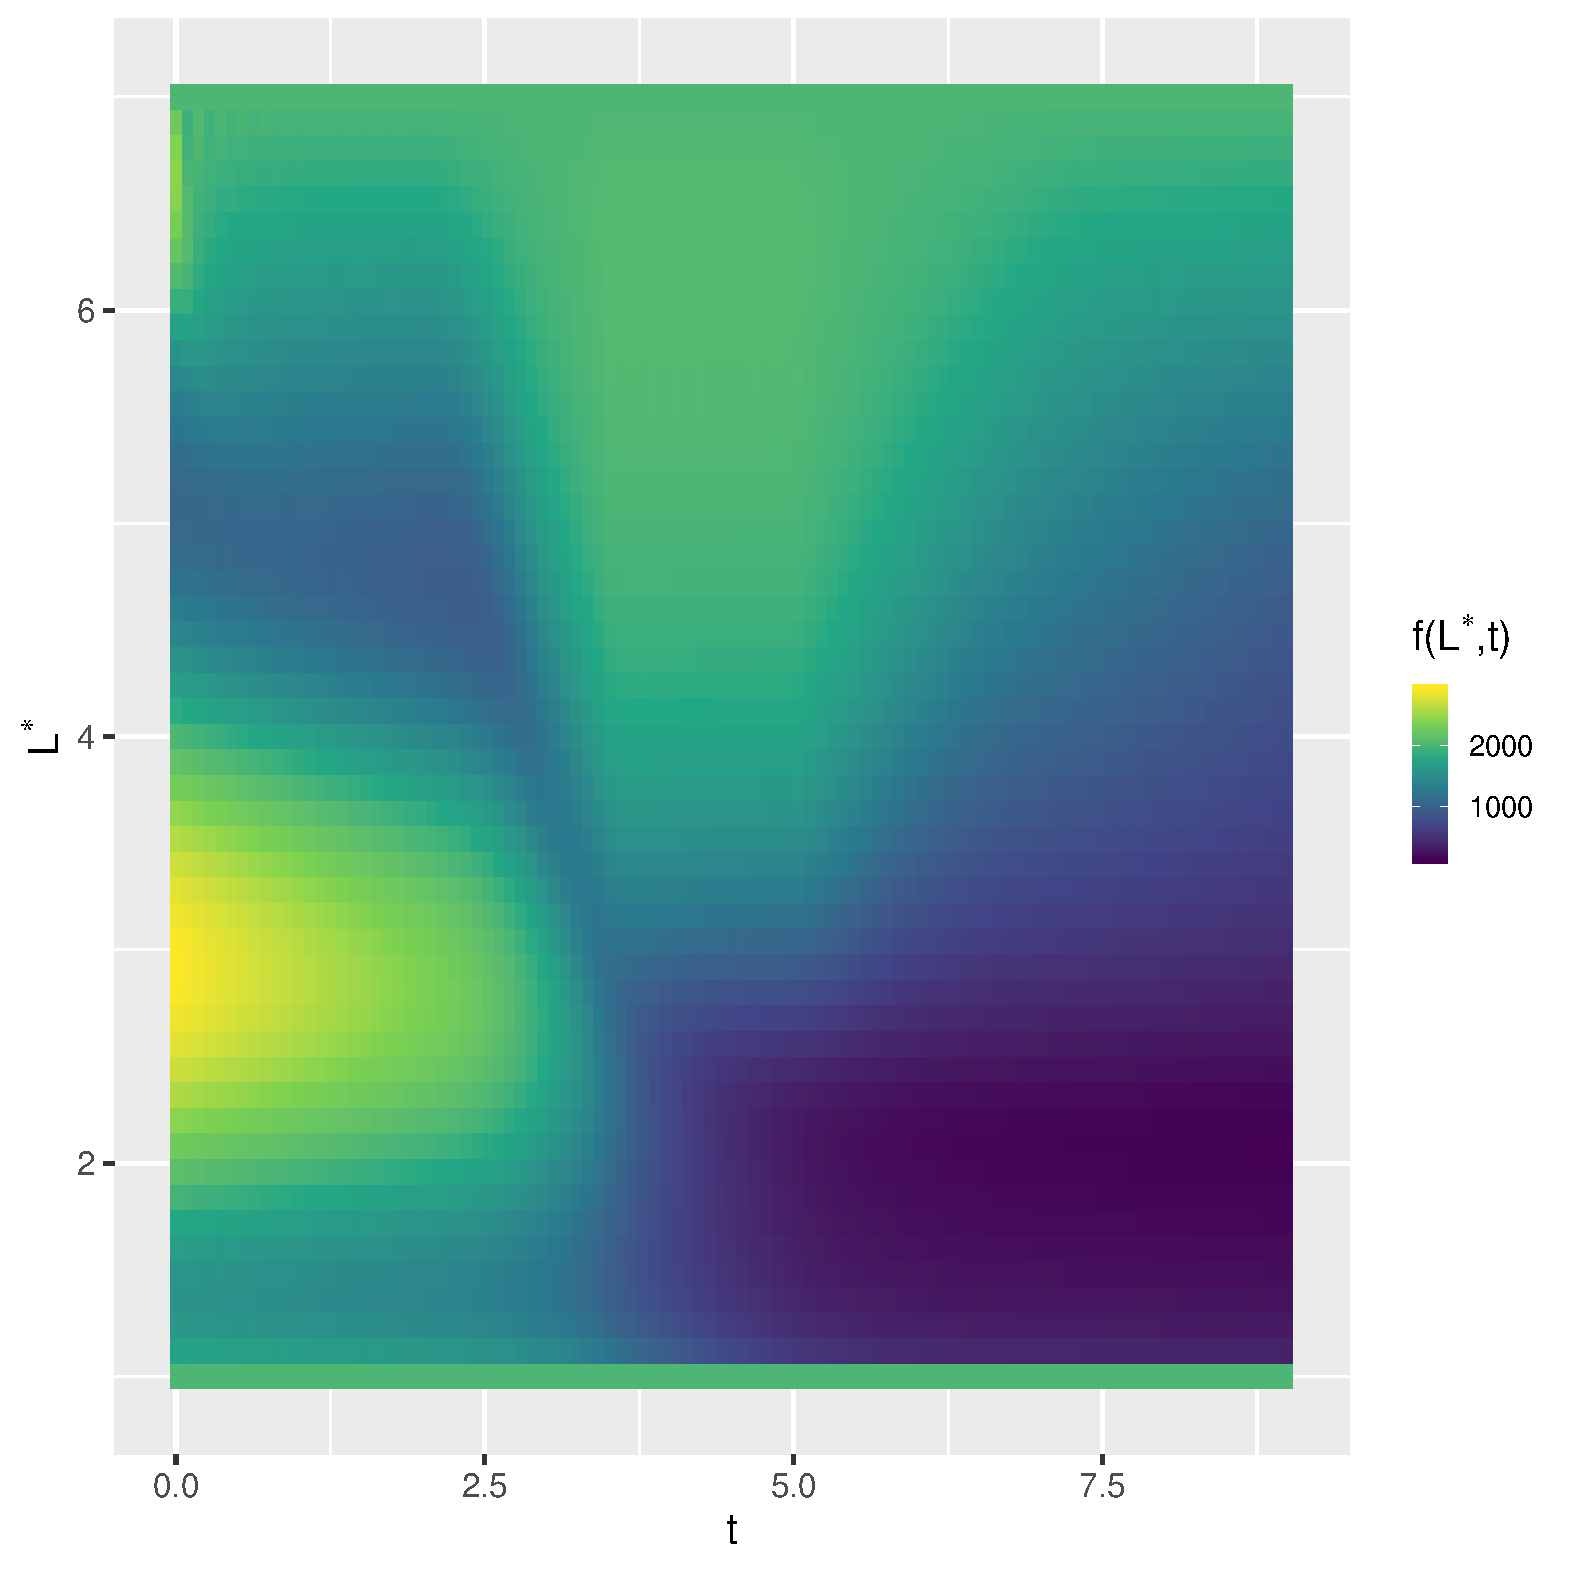
\includegraphics[width=0.75\textwidth]{psd.pdf}
    \caption{The radial diffusion solution.}
\end{figure}

\begin{figure}[ht]\label{fig:sensQTile}
    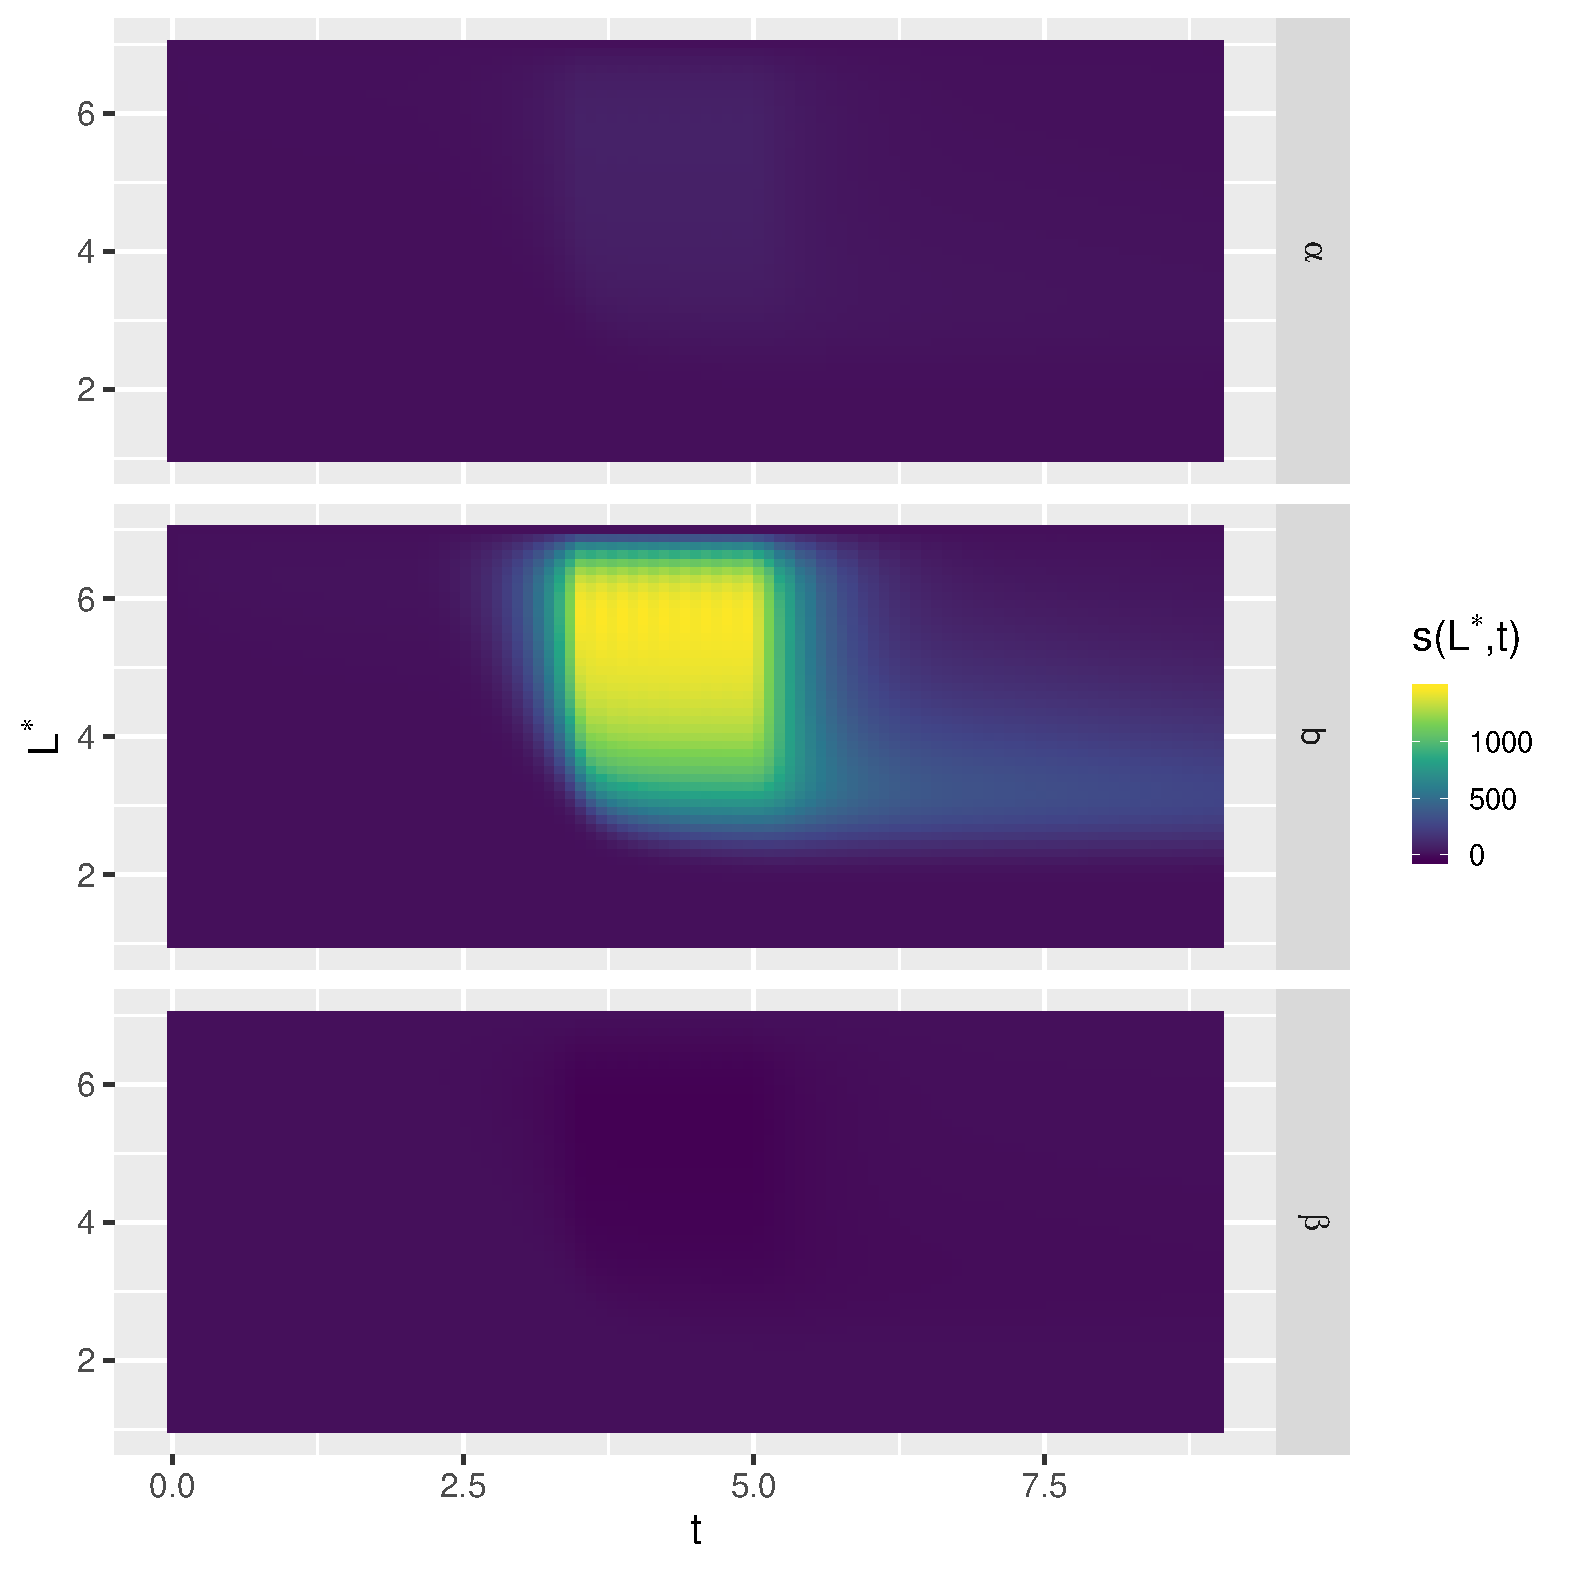
\includegraphics[width=0.75\textwidth]{sensitivity_Q.pdf}
    \caption{Sensitivity of the forward model to the parameters of the source term.}
\end{figure}

\begin{figure}[ht]\label{fig:sensRestTile}
    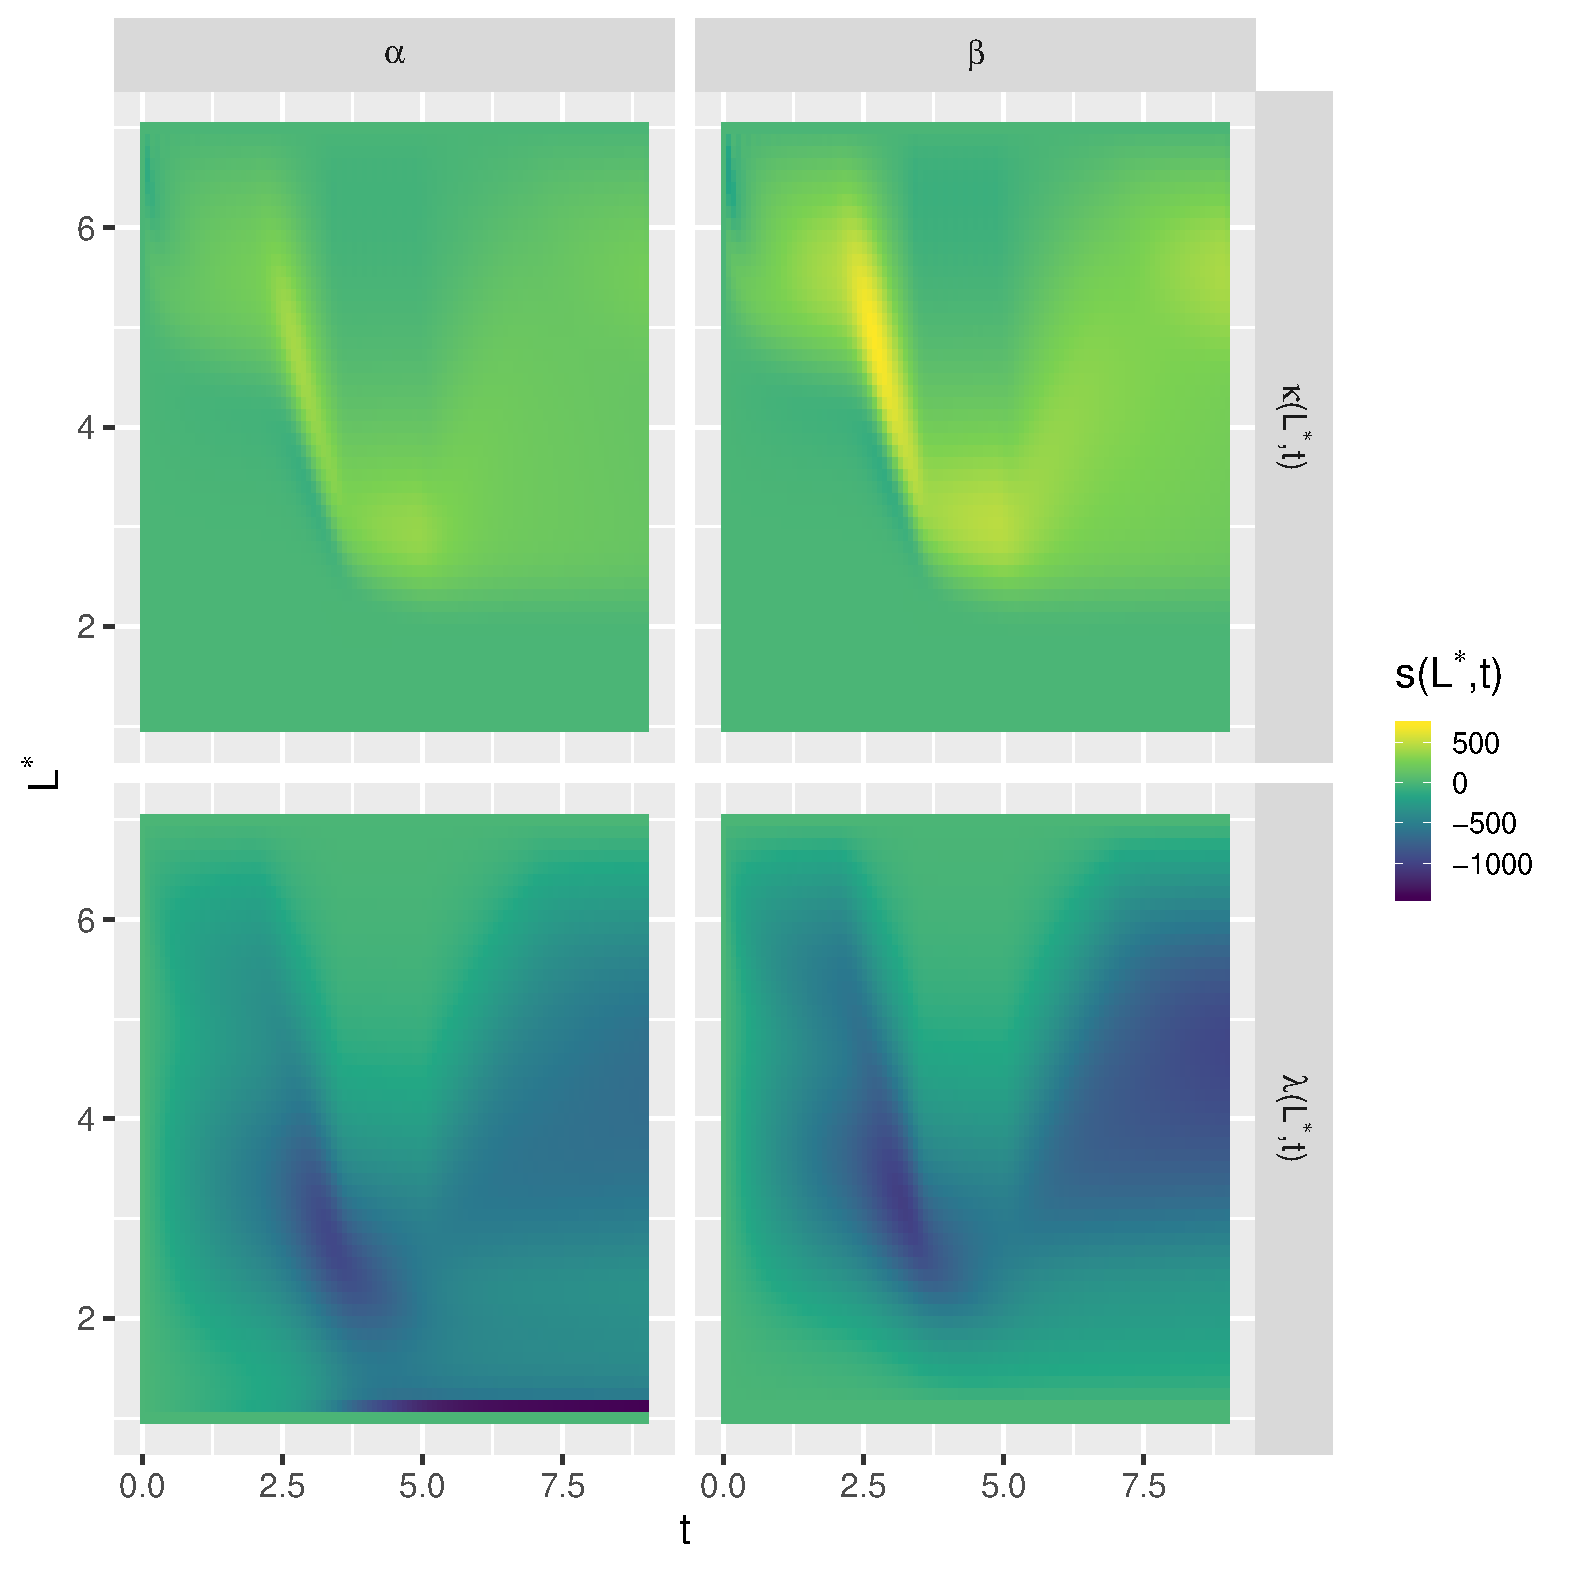
\includegraphics[width=0.75\textwidth]{sensitivity_rest.pdf}
    \caption{
        Sensitivity of the forward model to the parameters $\alpha$ and $\beta$ of 
        the diffusion field and loss rate.}
\end{figure}

\begin{figure}[ht]\label{fig:sensbTile}
    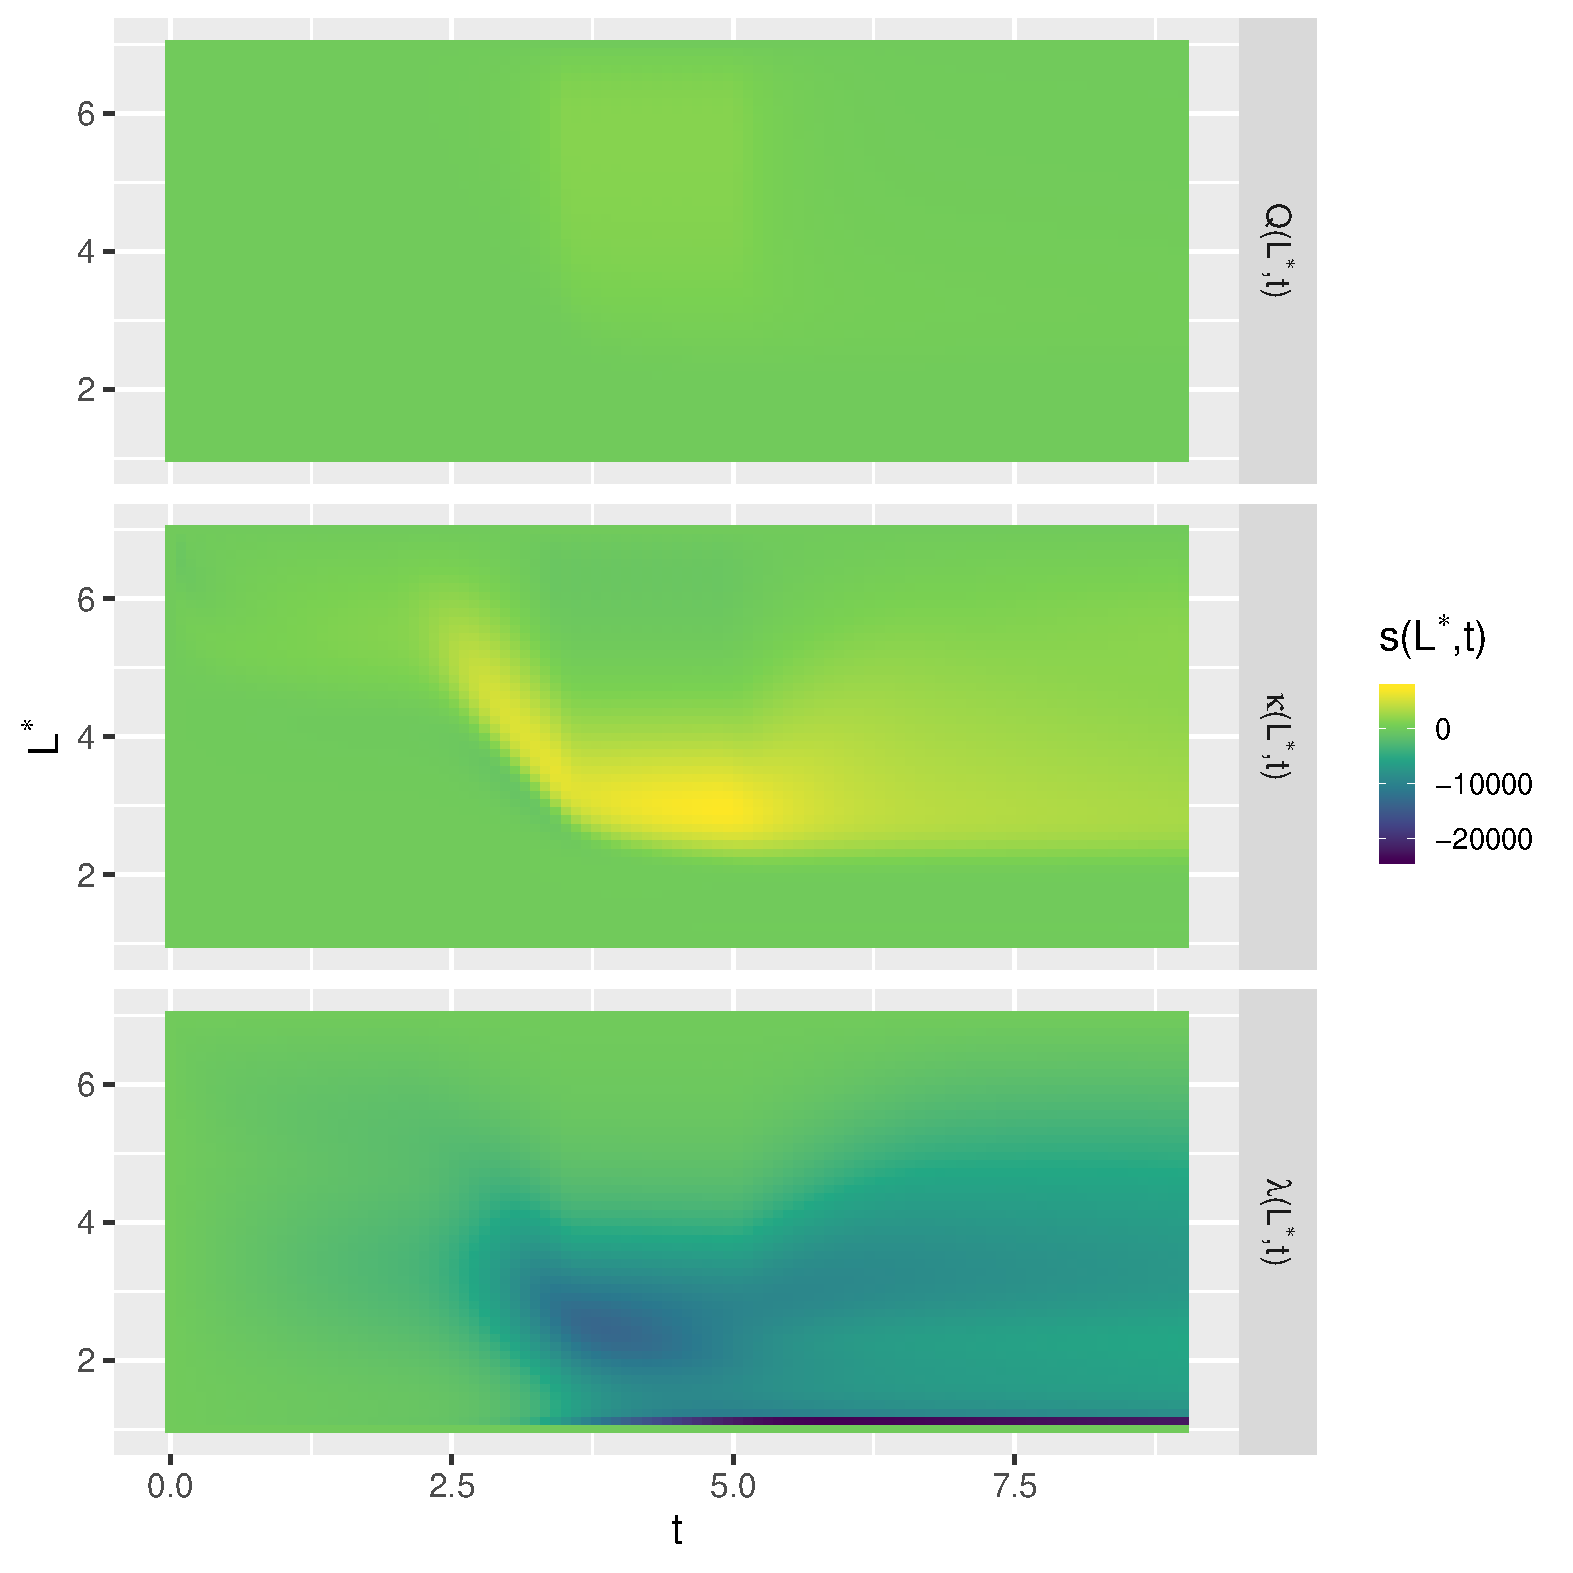
\includegraphics[width=0.75\textwidth]{sensitivity_b.pdf}
    \caption{
        Sensitivity of the forward model to the parameter $b$ of 
        the diffusion field, loss rate, and the source term.}
\end{figure}